In der Bildverarbeitung trifft man immer wieder auf den Begriff Deconvolution.
Wird ein Bild aufgenommen, entsteht zwangsläufig eine gewisse Unschärfe.
Mathematisch kann man dies als Faltung mit einer Pointspreadfunction verstehen
$$g(x,y) = f(x,y)*\operatorname{psf}(x,y),$$
wobei $g(x,y)$ das Originalbild und $f(x,y)$ das unscharfe Ergebnis der Aufnahme ist.
Den Prozess diese Faltung (engl. convolution) rückgängig zu machen nennt man deconvolution.
\begin{figure}[h]
\centering
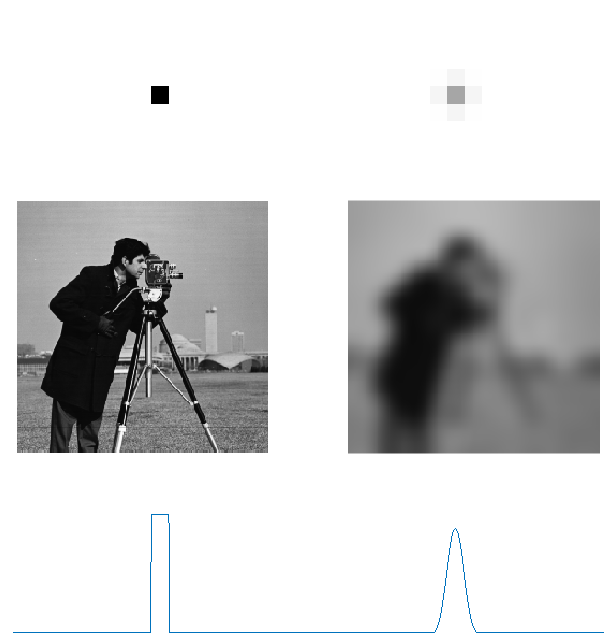
\includegraphics[width=0.9\textwidth]{./papers/deconvolve/pictures/psf.pdf}
\caption{Faltung mit Pointspreadfunction\label{deconvolve:pic}}
\end{figure}

In Abbildung \ref{deconvolve:pic} oben wird die Wirkung dieser Faltung auf ein einzelnes Pixel ersichtlich.
Betrachtet man nur eine Zeile davon, erkennt man wie die eckige Kurve \glqq verschmiert \grqq{} wird.
Aus einem scharfen Bild wird so ein unscharfes, wobei die Darstellung hier natürlich übertrieben ist.

In dieser Arbeit wird nun versucht, eine auf Wavelet basierte Methode zur Verbesserung der Bildschärfe zu entwerfen.
Begonnen wird hierbei mit einer eindimensionalen Funktion.
Das gleiche Vorgehen soll dann auf ein Bild angewendet werden.